\documentclass[aspectratio=169,13pt] {beamer}
%
% Choose how your presentation looks.
%
% For more themes, color themes and font themes, see:
% http://deic.uab.es/~iblanes/beamer_gallery/index_by_theme.html
%
\mode<presentation>
{
  \usetheme{Madrid}      % or try Darmstadt, Madrid, Warsaw, ...
  \usecolortheme{beaver} % or try albatross, beaver, crane, ...
  \usefonttheme{serif}  % or try serif, structurebold, ...
%  \setbeamertemplate{navigation symbols}{}
  \setbeamertemplate{caption}[numbered]
} 

\usepackage[,UTF8,linespread=1.2]{ctex}
\usepackage{wrapfig}
\usepackage{caption}
\captionsetup[figure]{name=图,labelsep=period}


\usepackage{xcolor}
\definecolor{xy_blue}{cmyk}{0.6,0.35,0.0,0.4}
\definecolor{xy_orange}{cmyk}{0.0,0.7,1.0,0.0}
\definecolor{xy_green}{cmyk}{0.2,0.0,1.0,0.15}
\xdefinecolor{xy_gold}{RGB}{135,103,79}
\xdefinecolor{xy2_gold}{cmyk}{0,0.35,0.75,0.05}
\usepackage{amsthm}

\newtheorem{peroration}{结论：}
\newtheorem{exploration}{探究：}
\newtheorem{prooft}{证明：}
\BeforeBeginEnvironment{peroration}{%
	\setbeamercolor{block title}{bg=xy_green,fg=white}
	\setbeamercolor{block body}{bg=xy_green!10}
}
\AfterEndEnvironment{peroration}{
	\setbeamercolor{block title}{bg=xy_blue,fg=white}
	\setbeamercolor{block body}{bg=xy_blue!10}
}
\BeforeBeginEnvironment{exploration}{%
	\setbeamercolor{block title}{bg=xy_orange,fg=white}
	\setbeamercolor{block body}{bg=xy_orange!10}
}
\AfterEndEnvironment{peroration}{
	\setbeamercolor{block title}{bg=xy_blue,fg=white}
	\setbeamercolor{block body}{bg=xy_blue!10}
}
\BeforeBeginEnvironment{solution}{%
	\setbeamercolor{block title}{bg=xy_green,fg=white}
	\setbeamercolor{block body}{bg=xy_green!10}
}
\AfterEndEnvironment{solution}{
	\setbeamercolor{block title}{bg=xy_green,fg=white}
	\setbeamercolor{block body}{bg=xy_green!10}
}
\BeforeBeginEnvironment{prooft}{%
	\setbeamercolor{block title}{bg=xy_green,fg=white}
	\setbeamercolor{block body}{bg=xy_green!10}
}
\AfterEndEnvironment{prooft}{
	\setbeamercolor{block title}{bg=xy_green,fg=white}
	\setbeamercolor{block body}{bg=xy_green!10}
}

\setbeamercolor{prooft}{fg=red, bg=green!10}       % 标题颜色
\setbeamercolor{prooft body}{fg=red, bg=red!5}  % 内容块背景
\setbeamerfont{prooft head}{series=\bfseries}       % 标题字体
\setbeamerfont{prooft body}{shape=\itshape}         % 内容字体
\renewcommand{\thefigure}{\arabic{figure}}

\title[2.2基本不等式]{2.2~~基本不等式}
\author[好好学习，努力向上]{}
\institute{}
\date{2026.9.22}
%\setbeamertemplate{theorems}[numbered]
\theoremstyle{definition}
\newtheorem{exam}{例}
\AtBeginSection[]
{
  \begin{frame}<beamer>
    \frametitle{本节主要内容}
    \tableofcontents[currentsection,currentsubsection]
  \end{frame}
}

\begin{document}
\begin{frame}{}
	\titlepage
\end{frame}

\begin{frame}{内容概览}
	\tableofcontents
\end{frame}

\section{前情回顾}
\begin{frame}{前情回顾}
	\begin{wrapfigure}{r}{4cm}
		\begin{center}		
			
\includegraphics{Figures/zhaoshuangxiantu.pdf}
			\caption{}
			\label{fig:zhaoshuang}
		\end{center}
	\end{wrapfigure}
	\hspace{2em}图 \ref{fig:zhaoshuang} 是在北京召开的第 24 届国际数学家大会的会标，会标是根据中国古代数学家赵爽的弦图设计的，颜色的明暗使它看上去像一个风车，代表中国人民热情好客。你能在这个图中找出一些相等关系和不等关系吗？
	
	\pause
	
	\begin{columns}
		
		\column{0.55\textwidth}
		\begin{peroration}<1->
			
			\hspace{2em} 一般地，$\forall \, a, b \in \mathbf{R}$，有
			\[
			\alert{ a^2+b^2 \geq 2ab},
			\]
			当且仅当 $a=b$ 时，等号成立.
		\end{peroration}
		\column{0.25\textwidth}
		
	\end{columns}
	
\end{frame}

\section{基本不等式}
\begin{frame}{基本不等式}
	当$a$，$b \in R_{\;+}$时，不等式
	\[
	\alert{ \sqrt{ab} \leqslant \dfrac{a+b}{2},\tag{1}}
	\]
	当且仅当$a=b$时，等号成立。
	
	不等式（1）称为基本不等式。
	
	其中，$\frac{a+b}{2}$叫做正数$a$，$b$的\alert{算术平均数}，
	
	$\sqrt{ab}$叫做正数$a$，$b$的\alert{几何平均数}。	
	
	
\end{frame}

\begin{frame}[t]
\frametitle{基本不等式的几何解释}	
\begin{columns}[t]
	\column{0.6\textwidth}

 \begin{exploration}
 	在图\ref{fig:average} 中，$AB$是圆的直径，点$C$是$AB$上一点，$AC=a$，$BC=b$，过点$C$作垂直于$AB$的弦$DE$，连接$AD$，$BD$。你能利用这个图形，得出基本不等式的几何解释吗？
 \end{exploration}
 
 \column{0.35\textwidth}
	\begin{figure}
	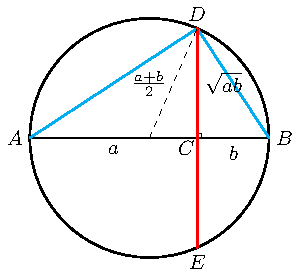
\includegraphics[scale=1]{Figures/average.pdf}
	\caption{}
	\label{fig:average}
	\end{figure}
\end{columns}
\end{frame}

\section{基本不等式的应用}

\begin{frame}[<+->][t]{求最值}
	\begin{exam}
		已知 $x>0$，求$x + \dfrac{1}{x}$的最小值。
	\end{exam}
	\begin{solution}
		因为$x>0$，所以
		\[
		 x+\frac{1}{x} \geqslant 2\sqrt{x\cdot \frac{1}{x}} =2
		 \]
		 当且仅当$x=\frac{1}{x}$，即$x^2=1$，$x=1$时，等号成立。因此所求的最小值为$2$。
	\end{solution}
\end{frame}

\begin{frame}[t]{求最值}
	\begin{exam}
		已知$x$、$y$都是正数，求证：
		\begin{enumerate}
			\item 如果积$xy$等于定值$P$，那么当$x=y$时，和$x+y$有最小值$2\sqrt{P}$；
			\item 如果和$x+y$等于定值$S$，那么当$x=y$时，积$xy$有最大值$\frac{1}{4}S^{\;2}$.
		\end{enumerate}
	\end{exam}
	

\end{frame}

\begin{frame}{证明I}
	
	\begin{prooft}
	因为$x$，$y$都是正数，所以
	\[ 
	\frac{x+y}{2}\geqslant \sqrt{xy},
	\]
	\begin{enumerate}
		\item 当积$xy$等于定值$P$时，
		\[
		\frac{x+y}{2} \geqslant \sqrt{P}
		\]
		所以
		\[
		x+y \geqslant 2\sqrt{P}
		\]
		当且仅当$x=y$时，上式等号成立。于是，当$x=y$时，和$x+y$有最小值$2\sqrt{P}$。
		
		
%		\item 当和$x+y$等于定值$S$时，
%		\[
%		\sqrt{xy} \leqslant \frac{S}{2},
%		\]
%		所以
%		\[
%		xy \leqslant \frac{1}{4}S^{\;2}.
%		\]
%		当且仅当$x=y$时，上式等号成立，于是，当$x=y$时，积$xy$有最大值$\frac{1}{4}S^{\;2}$。
	\end{enumerate}
\end{prooft}
\end{frame}

\begin{frame}{证明II}
	\BeforeBeginEnvironment{prooft}{%
		\setbeamercolor{block title}{bg=xy_green!10,fg=xy_green!10}
		\setbeamercolor{block body}{bg=xy_green!10}
%	\AfterEndEnvironment{prooft}{
%		\setbeamercolor{block title}{bg=xy_green,fg=white}
%		\setbeamercolor{block body}{bg=xy_green!10}
%		}
	}
	\begin{prooft}
		
	\begin{enumerate}
		\addtocounter{enumi}{1}
		
		\item 当和$x+y$等于定值$S$时，
		\[
		\sqrt{xy} \leqslant \frac{S}{2},
		\]
		所以
		\[
		xy \leqslant \frac{1}{4}S^{\;2}.
		\]
		当且仅当$x=y$时，上式等号成立，于是，当$x=y$时，积$xy$有最大值$\frac{1}{4}S^{\;2}$。
	\end{enumerate}
\end{prooft}
\end{frame}

\begin{frame}{布置作业}
	P46练习： 1---5
	
	P48 习题2.2：  1，2
\end{frame}

\end{document}
